%
% $RCSfile: microkernel.tex,v $
%
% Copyright (C) 2002-2008. Christian Heller.
%
% Permission is granted to copy, distribute and/or modify this document
% under the terms of the GNU Free Documentation License, Version 1.1 or
% any later version published by the Free Software Foundation; with no
% Invariant Sections, with no Front-Cover Texts and with no Back-Cover
% Texts. A copy of the license is included in the section entitled
% "GNU Free Documentation License".
%
% http://www.cybop.net
% - Cybernetics Oriented Programming -
%
% http://www.resmedicinae.org
% - Information in Medicine -
%
% Version: $Revision: 1.1 $ $Date: 2008-08-19 20:41:07 $ $Author: christian $
% Authors: Christian Heller <christian.heller@tuxtax.de>
%

\subsubsection{Microkernel}
\label{microkernel_heading}
\index{Microkernel Pattern}
\index{Internal Server}
\index{External Server}
\index{Daemon}
\index{Plug \& Play Environment}
\index{Operating System}
\index{OS}

The \emph{Microkernel} pattern \cite{buschmann} allows to keep a system flexible
and adaptable to changing requirements or new technologies. A minimal functional
\emph{Kernel} gets separated from extended functionality. The kernel may call
internal- or external servers (figure \ref{microkernel_figure}) to let them
solve special tasks which do not belong to its own core responsibility. Internal
servers, also called \emph{Daemons}, were already mentioned in section
\ref{local_process_heading}.

\begin{figure}[ht]
    \begin{center}
        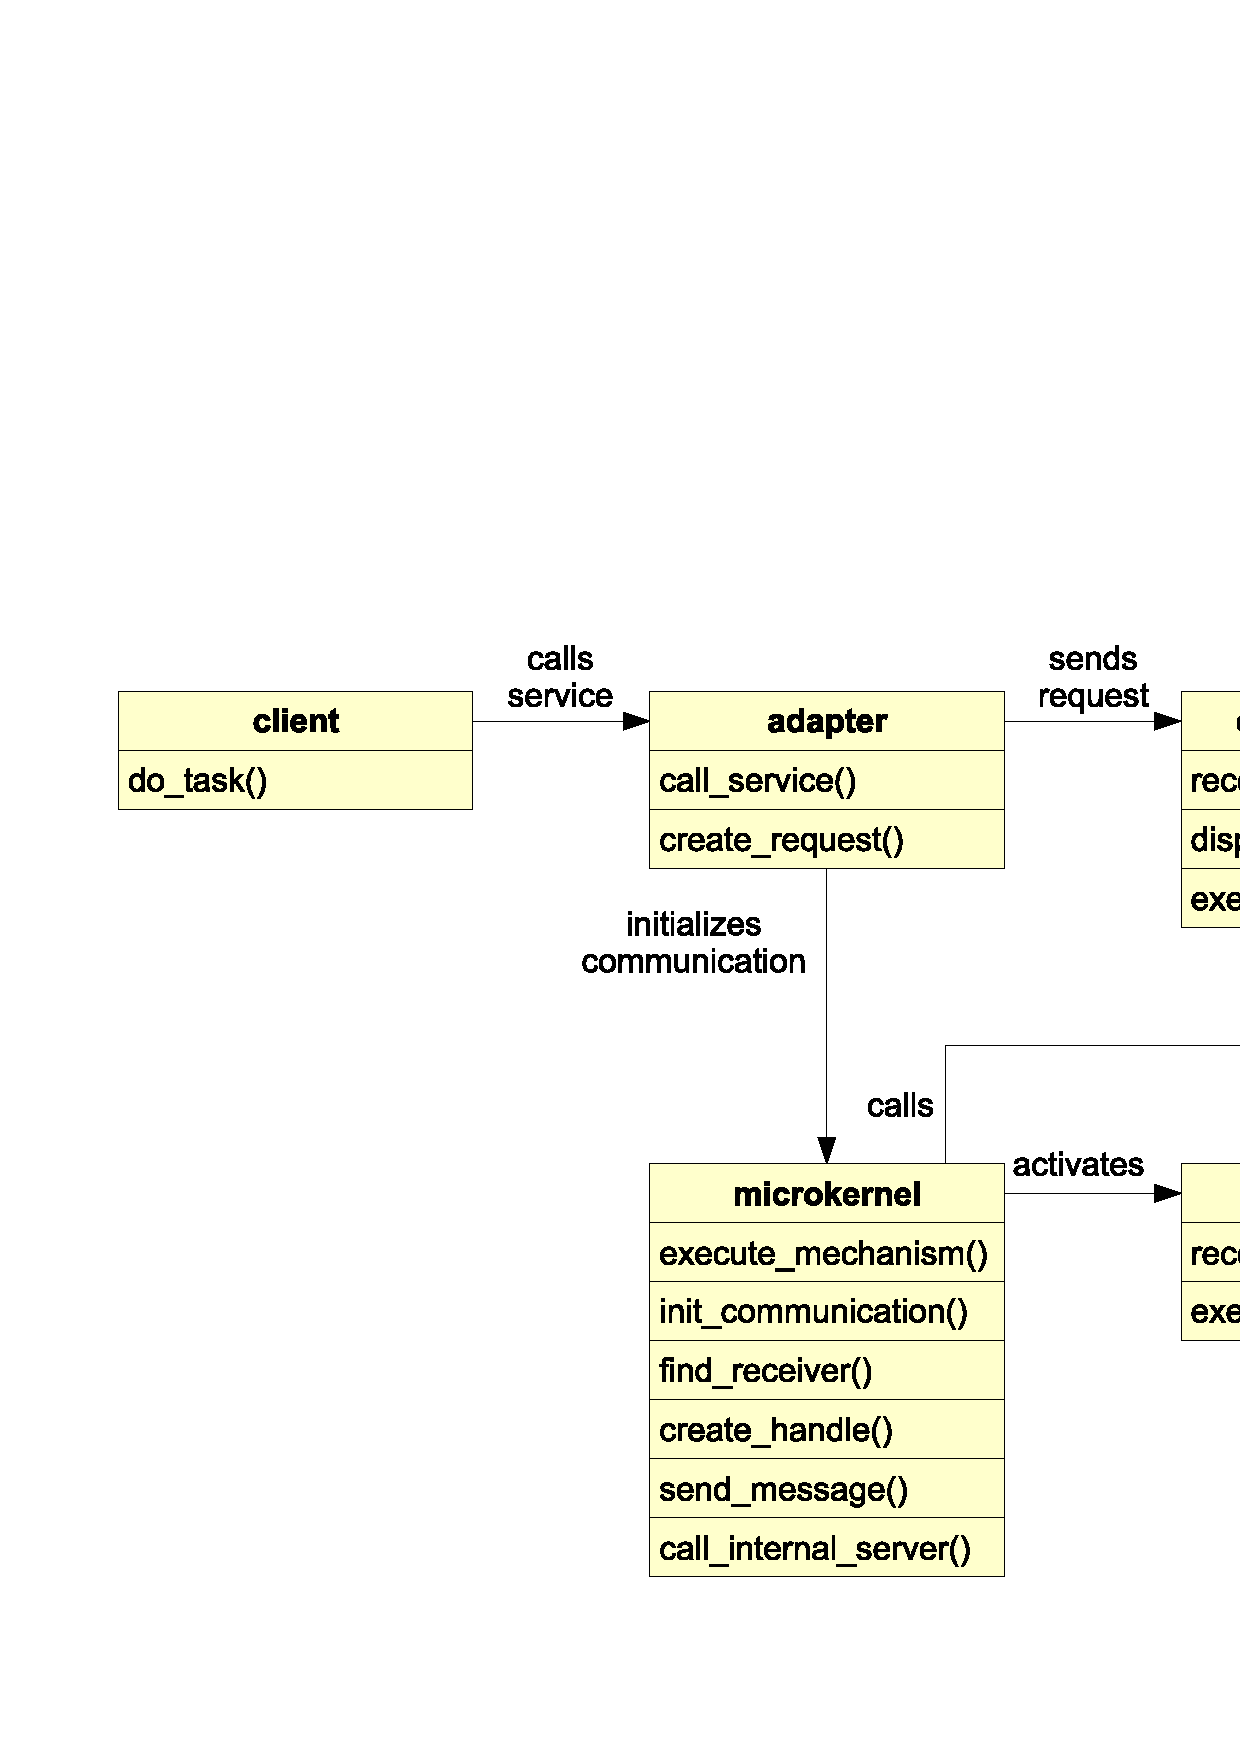
\includegraphics[scale=0.3,angle=-90]{graphic/microkernel.pdf}
        \caption{Microkernel Pattern}
        \label{microkernel_figure}
    \end{center}
\end{figure}

This pattern provides a \emph{Plug \& Play} environment and serves as base
architecture for many modern \emph{Operating Systems} (OS). Andrew S. Tanenbaum
recommends its use as well \cite{tanenbaum2001}. And also the interpreter that
will be described in chapter \ref{cybernetics_oriented_interpreter_heading}
uses this pattern in its own adapted form.

%
% CAUTION! This grpahics belongs to the 'broker.tex' file
% but was moved here for better formatting results in the document.
%

\begin{figure}[ht]
    \begin{center}
        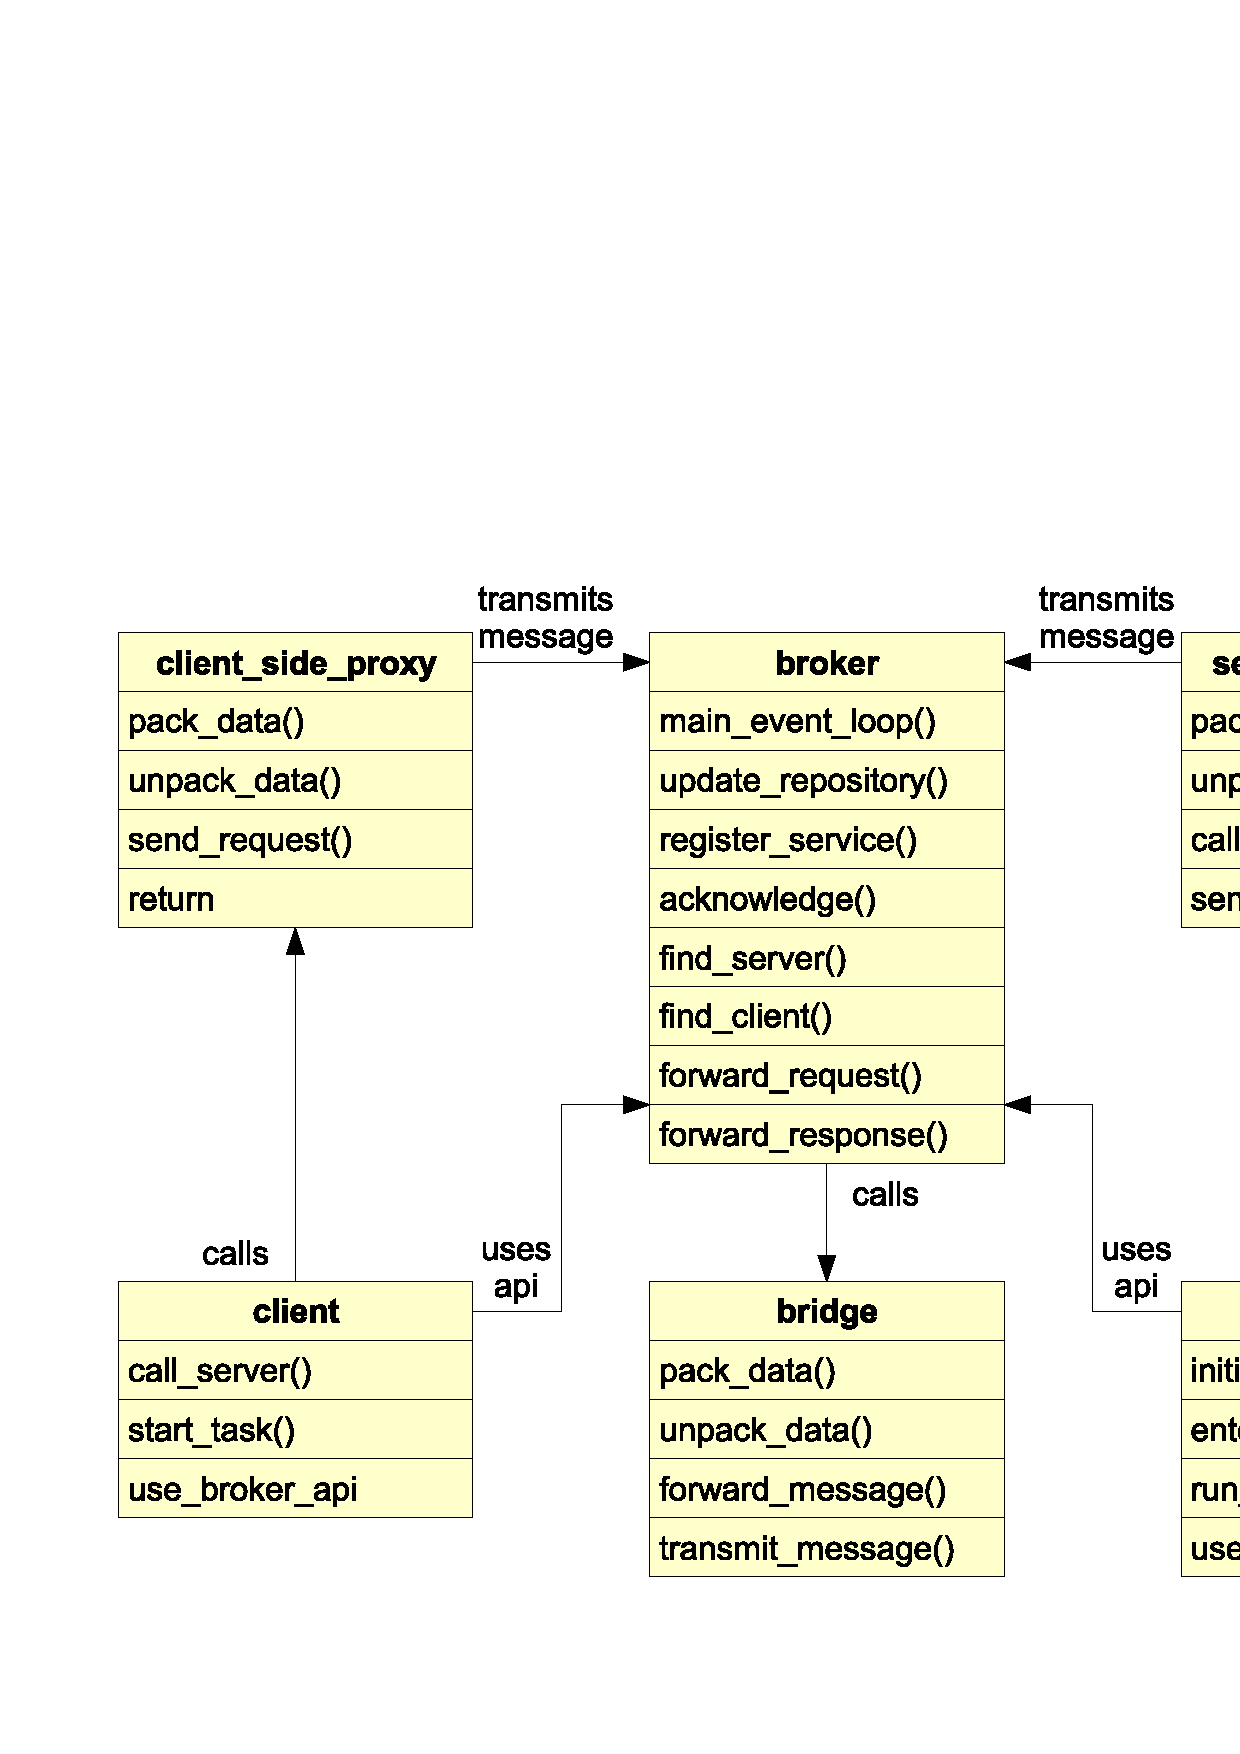
\includegraphics[scale=0.3,angle=-90]{graphic/broker.pdf}
        \caption{Broker Pattern}
        \label{broker_figure}
    \end{center}
\end{figure}

\clearpage
